\documentclass[tikz,border=5pt]{standalone}
\usetikzlibrary{arrows.meta}
\begin{document}
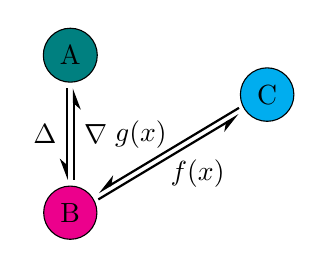
\begin{tikzpicture}[
    foo/.tip={Stealth[harpoon,swap]},
    mystyle/.style={thick, shorten >=2pt,shorten <=2pt},
]
    \node[draw,circle,fill=teal] (A) at (0,1) {A};
    \node[draw,circle,fill=magenta] (B) at (0,-1) {B};
    \node[draw,circle,fill=cyan] (C) at (2.5,.5) {C};

    \draw[-foo,mystyle,transform canvas={xshift=-0.3ex}] (A) -- node[left] {$\Delta$} (B);
    \draw[foo-,mystyle,transform canvas={xshift=+0.3ex}] (A) -- node[right] {$\nabla$} (B);
    % \draw[dualharpoon={$\Delta$}{$\nabla$}] (A) -- (B); % ?

    \draw[-foo,mystyle,transform canvas={yshift=-0.3ex}] (B) -- node[below right=-3pt] {$f(x)$} (C);
    \draw[foo-,mystyle,transform canvas={yshift=+0.3ex}] (B) -- node[above left=-3pt] {$g(x)$} (C);
    % \draw[dualharpoon={$f(x)$}{$g(x)$}] (B) -- (C); % ?
\end{tikzpicture}

\end{document}